\section{Argon Molecular Dynamics}

We can now apply these statistical ideas to the results of your argon MD simulation. Run as
long a simulation as is practical and make measurements of the temperature, potential energy
and the time average of the virial, which is given by
%
\begin{equation}
    \sum_i \sum_{j > i} r_{ij} \frac{ \partial V_{ij} }{ \partial r_{ij} }
\end{equation}
%
every MD time step. You should be able to run a few thousand steps, after thermalization.


\Question{} Measure the autocorrelation times for the temperature, potential energy and
virial.

\Answer{}
We run the Argon molecular dynamics from the last homework for a total \(24046\) steps,
and after \(15000\) steps we reached desired temperature (around \(1.0718\)).
Therefore, there are \(9047\) total steps for doing a statistical analysis.

We plot the potential energy, kinetic energy, and total energy in Figure~\ref{fig:MD_e_t},
which corresponds to the simulation time from \(t = 480\) to \(770\).

\begin{figure}[hb]
    \centering
    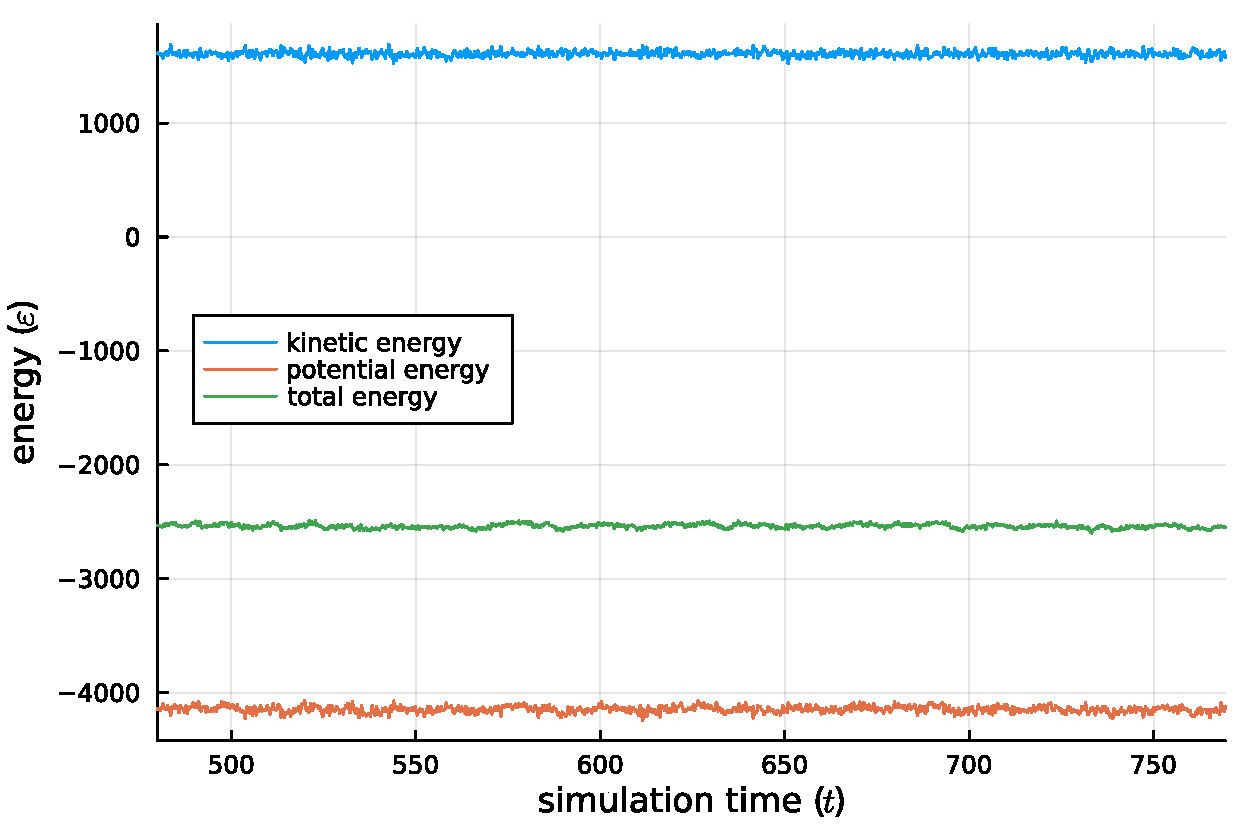
\includegraphics[width=0.8\textwidth]{e-t}
    \caption{The potential energy, kinetic energy, and total energy for the
        Argon molecular dynamics from simulation time from \(t = 480\) to \(770\).}
    \label{fig:MD_e_t}
\end{figure}

The temperature and virial terms are plotted in
Figure~\ref{fig:MD:a} and Figure~\ref{fig:MD:b}, respectively.

\begin{figure}[H]
    \centering
    \begin{minipage}[t]{0.8\linewidth}
        \centering
        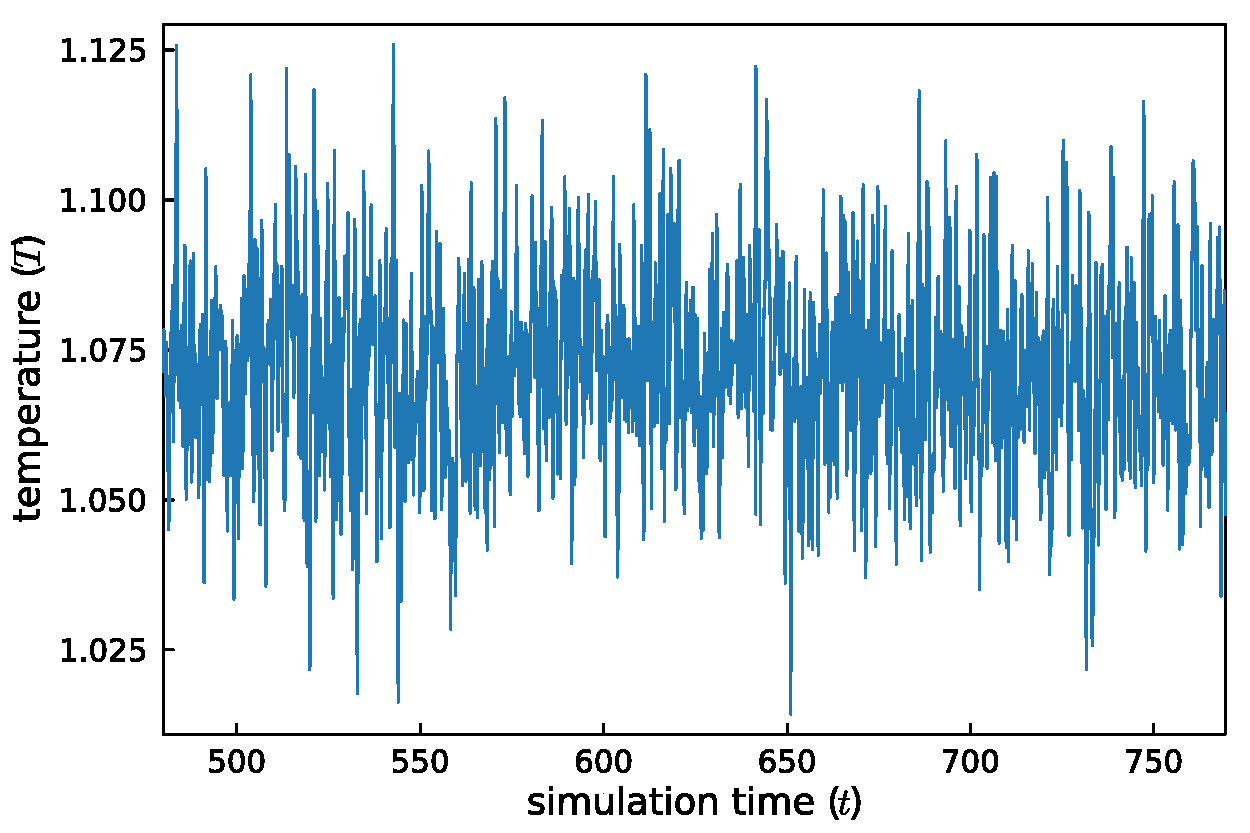
\includegraphics[width=\linewidth]{MD_temperature}
        \subcaption{The temperature for the
            Argon molecular dynamics from simulation time from \(t = 480\) to \(770\).}
        \label{fig:MD:a}
    \end{minipage}
    \hfill
    \begin{minipage}[t]{0.8\linewidth}
        \centering
        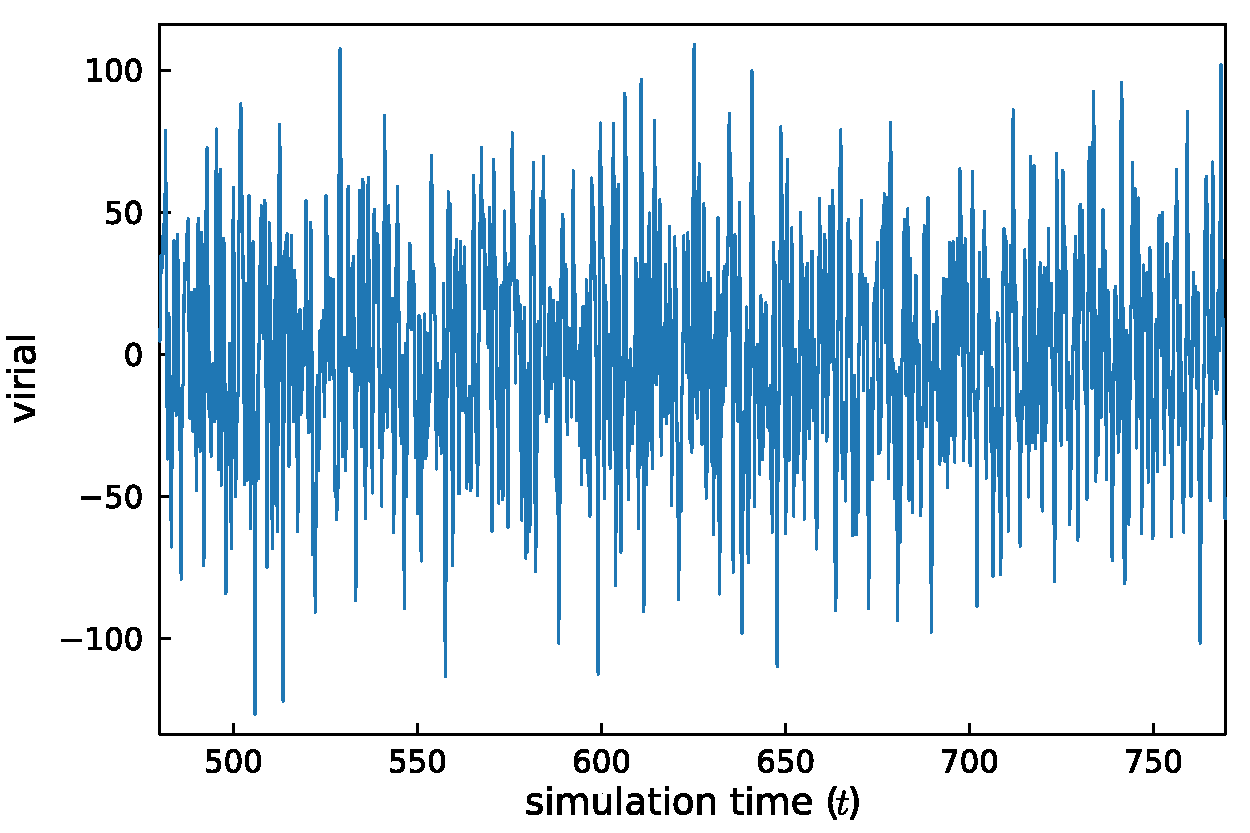
\includegraphics[width=\linewidth]{MD_virial}
        \subcaption{The virial for the
            Argon molecular dynamics from simulation time from \(t = 480\) to \(770\).}
        \label{fig:MD:b}
    \end{minipage}
    \caption{The temperature and virial terms for the
        Argon molecular dynamics.}
    \label{fig:MD}
\end{figure}


\Question{} Also measure the covariance matrix for these \(3\) quantities.

\Answer{}



\Question{} Use your estimate of the autocorrelation times, along with binning and the
jackknife method to give an error on the pressure from your simulation.

\Answer{}

